\chapter{Algoritmi deterministici}



% TODO: Estendere a MaxMatching?
\section{\BiMaxMatching}\label{sec:BiMaxMatching}
Sia $G=(V,E)$ un grafo non orientato. Un \emph{matching} (matrimonio) in $G$ è una selezione di lati in $E$ tale che su nessun vertice in $V$ incide più di un lato.
\MaxMatching è il problema di trovare il matching di cardinalità massima in un dato grafo.

\BiMaxMatching è una versione di \MaxMatching su grafi bipartiti, cioè in cui i vertici sono divisi in due classi e ogni lato incide su un vertice per classe: $G=(V_1,V_2,E)$ dove $V_1\cup V_2=\emptyset$ e $E\subseteq V_1\times V_2$. $\BiMaxMatching\in\PO$.

\popt{\BiMaxMatching}
{Grafo bipartito $G=(V_1,V_2,E)$}
{$X\subseteq E$}
{Determinare il matching di cardinalità massima in $G$}
{$X\subseteq E$}
{$\MAX$}
{$\card X$}

\begin{figure}
	\centering
	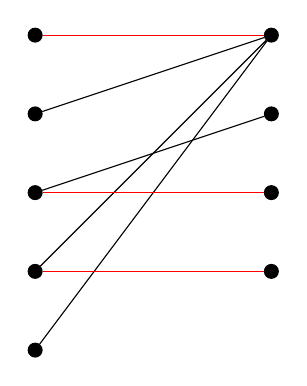
\begin{tikzpicture}
	\node[draw,inner sep=0pt,minimum size=5pt,fill, circle] at (0, 1)  (a) {};
	\node[draw,inner sep=0pt,minimum size=5pt,fill, circle] at (0, 2)  (b) {};
	\node[draw,inner sep=0pt,minimum size=5pt,fill, circle] at (0, 3)  (c) {};
	\node[draw,inner sep=0pt,minimum size=5pt,fill, circle] at (0, 4)  (d) {};
	\node[draw,inner sep=0pt,minimum size=5pt,fill, circle] at (0, 5)  (e) {};

	\node[draw,inner sep=0pt,minimum size=5pt,fill, circle] at (3, 2)  (f) {};
	\node[draw,inner sep=0pt,minimum size=5pt,fill, circle] at (3, 3)  (g) {};
	\node[draw,inner sep=0pt,minimum size=5pt,fill, circle] at (3, 4)  (h) {};
	\node[draw,inner sep=0pt,minimum size=5pt,fill, circle] at (3, 5)  (i) {};

	\draw (a) -- (i);
	\draw (b) -- (i);
	\draw (d) -- (i);
	\draw[red] (e) -- (i);
	\draw[red] (b) -- (f);
	\draw[red] (c) -- (g);
	\draw (c) -- (h);
\end{tikzpicture}

	\caption{Esempio di grafo bipartito. I lati colorati rappresentano un possibile matching.}
	\label{fig:graphmatching}
\end{figure}

Fissato un matching $M\subseteq E$, un lato $l\in E$ si dice \emph{occupato} se $l\in M$ e \emph{libero} se $l\notin M$.
Un vertice si dice \emph{esposto} se e solo se su di esso incidono solo lati liberi. Un cammino semplice si dice \emph{aumentante} rispetto a un matching se alterna lati liberi e occupati e inizia e termina su vertici esposti.
Quando un matching ha un cammino aumentante si può fare un \flang{flip}, cioè invertire l'appartenenza al matching dei lati del cammino aumentante.

\begin{figure}
	\centering
	\begin{subfigure}[b]{0.4\textwidth}
		\centering
		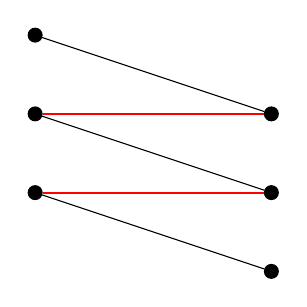
\begin{tikzpicture}[every node/.style={draw,inner sep=0pt,minimum size=5pt,fill,circle},matching/.style={red,thick}]
	\node at (3,1) (a) {};
	\node at (0,2) (b) {};
	\node at (0,3) (c) {};
	\node at (3,2) (f) {};
	\node at (3,3) (g) {};
	\node at (0,4) (h) {};

	\draw		(a) -- (b);
	\draw[matching]	(b) -- (f);
	\draw		(f) -- (c);
	\draw[matching]	(c) -- (g);
	\draw		(g) -- (h);
\end{tikzpicture}

		\subcaption{Prima del flip.}
	\end{subfigure}
	\begin{subfigure}[b]{0.4\textwidth}
		\centering
		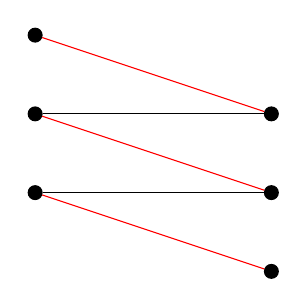
\begin{tikzpicture}
	\node[draw,inner sep=0pt,minimum size=5pt,fill, circle] at (3, 1)  (a) {};
	\node[draw,inner sep=0pt,minimum size=5pt,fill, circle] at (0, 2)  (b) {};
	\node[draw,inner sep=0pt,minimum size=5pt,fill, circle] at (0, 3)  (c) {};
	\node[draw,inner sep=0pt,minimum size=5pt,fill, circle] at (3, 2)  (f) {};
	\node[draw,inner sep=0pt,minimum size=5pt,fill, circle] at (3, 3)  (g) {};
	\node[draw,inner sep=0pt,minimum size=5pt,fill, circle] at (0, 4)  (h) {};

	\draw[red] (a) -- (b);
	\draw (b) -- (f);
	\draw[red] (f) -- (c);
	\draw (c) -- (g);
	\draw[red] (g) -- (h);
\end{tikzpicture}

		\subcaption{Dopo il flip.}
	\end{subfigure}
	\caption{Esempio di cammino aumentante in un grafo bipartito.}
	\label{fig:augpaths}
\end{figure}

Vale il seguente teorema relativo ai cammini aumentanti per matching su grafi:
\begin{theorem}
	Sia $M$ un matching per un grafo $G$. Allora:
	\begin{equation*}
		\text{Esiste un cammino aumentante per $M$} \iff \text{$M$ non è massimo per $G$.}
	\end{equation*}
\end{theorem}
\begin{proof}~
	\begin{description}
		\item[$\Rightarrow$)] Applicando un flip al cammino aumentante si aumenta il matching di $1$.
		\item[$\Leftarrow$)] Se $M$ non è massimo, sia $M'$ il matching massimo per $G$ e sia $X:=(M\setminus M')\cup(M'\setminus M)$ (la differenza simmetrica di $M$ e $M'$).
			Su ogni vertice di $G$ possono incidere al più $2$ lati di $X$ (uno per ciascuno dei due matching).
			Nel grafo indotto da $X$, in ogni circuito l'appartenenza dei lati a $M$ e $M'$ è alternata e quindi il circuito è composto dallo stesso numero di lati di $M$ e di $M'$.
			Siccome però $M'$ ha più lati di $M$, esiste almeno un cammino semplice nel grafo indotto da $X$ che ha più lati in $M'$.
			Tale cammino alterna lati di $M$ e di $M'$ ed è aumentante rispetto a $M$ in $G$.
	\end{description}
\end{proof}

% TODO: è necessario discutere di come viene effettuata la visita per FindAugmenting e quale sia la sua complessità. Tenere conto di ciò nel paragone con MaxMatching: è possibile usare lo stesso algoritmo su grafi non bipartiti?
\SetKwFunction{FindAugmenting}{FindAugmenting}
\SetKwFunction{Flip}{Flip}
L'algoritmo \ref{alg:BiMaxMatching} risolve \BiMaxMatching trovando l'ottimo in tempo polinomiale.
La procedura \FindAugmenting tiene traccia dei vertici esposti e fa una visita in profondità del grafo a partire da uno di essi, alternando lati liberi e occupati, identificando un cammino aumentante.
La procedura \Flip esegue un flip del matching dato.

\begin{algorithm}
	$M \asn \emptyset$\;
\While{}{
	$\pi\asn\FindAugmenting{G,M}$\;
	\If{$\pi=\bot$}{
		\Return $M$\;
	}\Else{
		$M\asn\Flip(M,\pi)$\;
	}
}

	\caption{Risoluzione polinomiale di \BiMaxMatching}
	\label{alg:BiMaxMatching}
\end{algorithm}

\begin{corollario}
	$\BiMaxMatching\in\PO$.
\end{corollario}

\PerfectMatching è il problema di decisione che si chiede se in un grafo bipartito esista un matching che coinvolge tutti i vertici.

\begin{corollario}
	$\PerfectMatching\in\P$.
\end{corollario}



\section{\LoadBalancing}
Il problema \LoadBalancing (bilanciamento del carico) consiste nel dividere un insieme di task, ciascuno con la sua durata, tra le macchine di un insieme, in modo da minimizzare la durata complessiva (carico) impiegata dalla macchina più lenta. Questo problema è \NPO-completo.

\popt
{\LoadBalancing}
{Durate $t_0,\dots,t_{n-1}\in\N^+$ per $n$ task, numero $m$ di macchine}
{Assegnamento di ciascun task a una macchina}
{Determinare l'assegnamento che minimizza la durata massima}
{Assegnamenti $x:n\to m$}
{$\MIN$}
{$L=\max_j L_j$, dove $L_j:=\sum_{i\in x^{-1}(j)} t_i$}


\subsection{\GreedyLoadBalancing}
Un algoritmo greedy può trovare una soluzione ammissibile per \LoadBalancing.
L'algoritmo esamina i task $t_0,t_1,\dots,t_{n-1}$ nell'ordine, assegnando ogni task alla macchina più scarica.
\GreedyLoadBalancing, se implementato con una coda con priorità che tenga conto della macchina dal carico minimo (effettuando $n$ operazioni di insert/update per i carichi di $m$ macchine), opera in tempo $O(n\log m)$.
L'algoritmo non ottiene, in generale, la soluzione ottima, ma ha la garanzia di non produrre più del doppio dell'ottimo, come dimostrato dal seguente teorema:

\begin{theorem}\label{thm:greedyloadbalancing}
	\GreedyLoadBalancing è un algoritmo 2-approssimante per \LoadBalancing.
\end{theorem}
Prima di dimostrare il teorema si consideri il seguente lemma:
\begin{lemma}\label{lem:load:ultimopasso}
	Sia $L\star$ il costo della soluzione ottima. Sia $\bar j$ tale che $L_{\bar j}=L\star$ e sia $\bar i$ l'ultimo task assegnato a $\bar j$. Allora:
	\begin{equation*}
		L_{\bar j}-t_{\bar i} \leq L\star
	\end{equation*}
\end{lemma}
\begin{proof}
	Il carico della macchina $\bar j$ prima dell'assegnamento $\bar i$ era $L_{\bar j}-t_{\bar i}$, il cui era minore di ogni altro carico per via di come l'algoritmo sceglie a chi assegnare.
	Indicato con $L\star_j$ il carico della macchina $j$ nella soluzione ottima, vale $L\star\geq\frac1m\sum_it_i$, essendo $mL\star\geq\sum_jL\star_j=\sum_it_i$.
	\begin{gather*}
		L_{\bar j}-t_{\bar i}\leq L_j \qquad\forall j \\
		\sum_j (L_{\bar j}-t_{\bar i})\leq\sum_j L_j=\sum_i t_i\\
		m(L_{\bar j}-t_{\bar i})\leq \sum_i t_i \\
		L_{\bar j}-t_{\bar i}\leq\frac1m\sum_j t_j\leq L\star
	\end{gather*}
\end{proof}
Si può ora procedere con la dimostrazione del teorema \ref{thm:greedyloadbalancing}:
\begin{proof}
	Si osservi che $L\star\geq\max_it_i$. Applicando il lemma \ref{lem:load:ultimopasso}:
	\begin{gather*}
		L=L_{\bar j}=\underbrace{L_{\bar j}-t_{\bar i}}_{\leq L\star}+\underbrace{t_{\bar i}}_{\leq L\star}\leq 2L\star \\[1ex]
		\frac L{L\star}\leq 2
	\end{gather*}
\end{proof}

\begin{corollario}
	$\LoadBalancing\in\gAPX2$.
\end{corollario}

Si dimostra che questo risultato sull'analisi di \GreedyLoadBalancing è tight:
\begin{theorem}
	Per ogni $\varepsilon>0$ esiste un input di \LoadBalancing su cui \GreedyLoadBalancing produce una soluzione $L$ tale che
	\begin{equation*}
		2-\varepsilon\leq\frac L{L\star}\leq2
	\end{equation*}
\end{theorem}
\begin{proof}
	Scegliamo un numero di macchine $m>\frac1\varepsilon$ e un numero di task $n=m(m-1)+1$. Questi task consistono, nell'ordine, in $n-1$ task da $1$ e un task da $m$. Naturalmente la soluzione ottima assegna unicamente il task da $m$ a una macchina, che risulta la più carica, quindi $L\star=m$.

	Per assegnare i task, l'algoritmo assegna un task da $1$ per ogni macchina ciclicamente finché arriva il task da $m$, che viene assegnato a una macchina di carico $m-1$ producendo un costo finale di $2m-1$. In questo caso si ha
	\begin{equation*}
		\frac L{L\star}=\frac{2m-1}{m}=2-\frac1m\geq2-\varepsilon
	\end{equation*}
\end{proof}


\subsection{\SortedGreedyBalance}
Un algoritmo \SortedGreedyBalance può ordinare i task in ordine decrescente prima di assegnarli come \GreedyLoadBalancing. Questo algoritmo ha costo in tempo di $O(n\log n+n\log m)$.

\begin{theorem}
	\SortedGreedyBalance è un algoritmo $\frac32$-approssimante per \LoadBalancing.
\end{theorem}
\begin{proof}
	Se $n\leq m$ la soluzione è ottima e la tesi è ovvia.

	Se $n>m$, esiste una macchina che riceve due task. Il primo task assegnato a una macchina già carica è $t_m$, e vale:
	\begin{equation*}
		L\star\geq 2t_m
	\end{equation*}

	Sia $\bar j$ la macchina con carico massimo al termine dell'esecuzione e $\bar i$ l'ultimo carico assegnato. Si ha $\bar i \geq m$, da cui $t_{\bar i}\leq t_m$ e quindi $t_{\bar i}\leq t_m\leq \frac12 L\star$.
	\begin{gather*}
		L=\underbrace{L_{\bar j}-t_{\bar i}}_{\leq L\star}+\underbrace{t_{\bar i} }_{\leq \frac12 L\star}\leq L\star+\frac12 L\star=\frac32L\star
	\end{gather*}
\end{proof}

Valgono inoltre i seguenti teoremi riguardanti \LoadBalancing, che non dimostriamo.
\begin{theorem}~
	\begin{itemize}
		% TODO: add bib
		\item \SortedGreedyBalance è un algoritmo $\frac43$-approssimante per \LoadBalancing \cite{Graham:69:sortedgreedybalance};
		\item $\LoadBalancing\in\PTAS$;
		\item $\P\neq\NP\impl\LoadBalancing\notin\FPTAS$.
	\end{itemize}
\end{theorem}



\section{\CenterSelection}
Nel problema \CenterSelection è dato uno spazio metrico $\tuple{S,d}$ di punti.
Si vuole minimizzare la distanza massima $\rho(C)$ tra un nodo e il suo nodo di riferimento, detta raggio di copertura.
\CenterSelection è un problema \NPO-completo.

\popt{\CenterSelection}
{Insieme $S$ di punti, metrica $d$, numero massimo di centri $k\in\N^+$}
{Centri $C\subseteq S$}
{Quali centri selezionare in modo da minimizzare il raggio di copertura}
{$C\subseteq S\mid \card C\leq k$}
{$\MIN$}
{$\rho(C) = \max_{x \in S} d(x, C)$}

Uno spazio metrico è un insieme $\Omega$ di punti su cui vale una funzione distanza $d:\Omega\times\Omega\to\R^{\geq0}$ tale che:
\begin{itemize}
	\item $d(x,y)=0\iff x=y$
	\item $d(x,y)=d(y,x)\forall x,y\in\Omega$
	\item $d(x,y)=d(x,z)+d(z,y)$ (disuguaglianza triangolare)
\end{itemize}

\begin{defin}[tassellificazione di Voronoi]
	Dato uno spazio metrico $\tuple{\Omega,d}$, sia $S\subseteq\Omega$ finito e $C\subseteq S$ l'insieme dei centri. Per ogni $c\in C$ la cella di Voronoi rispetto al centro $c$ è l'insieme dei punti $s\in S$ tali che
	\begin{equation*}
		c=\arg\min_{c'\in C} d(s,c')
	\end{equation*}
	% TODO: brutta, esprimere meglio
	Dato un punto $s\in S$ definiamo l'assegnamento di $s$ alla cella di centro $c\in C$ $\text{VC}_C(s)=\arg\min_{c'\in C} d(s,c')$.
\end{defin}

\begin{equation*}
	\text{VC}_C(s)=\arg\min_{c\in C} d(s,c)
\end{equation*}

\CenterSelection è il problema che riceve in input $S\subseteq_\text{fin}\Omega$ e $k\in\N^+$, ha come soluzioni ammissibili le selezioni di centri $C\subseteq S$ con $\card C\leq k$ e come obiettivo da minimizzare:
\begin{equation*}
	\rho(C)=\max_{s\in S} d(s,\text{VC}_C(s))
\end{equation*}

\subsection{\CenterSelectionPlus}
L'algoritmo \ref{alg:CenterSelectionPlus} non risolve \CenterSelection in quanto richiede un input $r$ aggiuntivo rispetto a quelli previsti dal problema, che consiste in una stima del raggio di copertura ottimo $r\star$.

\begin{algorithm}[ht]
	\caption{\CenterSelectionPlus}
	\label{alg:CenterSelectionPlus}
	\SetKwFunction{ExtractRandomPoint}{ExtractRandomPoint}

\KwInput{$S$, $k$, $d$, $r$}

$C\asn\emptyset$\;
\While{$S \neq \emptyset$}{
	$\bar s\asn\ExtractRandomPoint(S)$\;
	$C\asn C\cup \set{\bar s}$\;
	$S\asn S\setminus\set{x\mid d(x,\bar s)\leq 2r}$\;
}
\If{$\card C\leq k$}{
	\Return $C$\;
}\Else{
	Impossibile\;
}

\end{algorithm}

Si noti che un algoritmo \CenterSelectionPlus' che, invece di eliminare punti di $S$, non prenda in considerazione nella selezione di nuovi centri punti $s$ tali che $d(s,C)>2r$, è del tutto equivalente a \CenterSelectionPlus.
\begin{theorem}
	Valgono le seguenti proprietà per \CenterSelectionPlus:
	\begin{enumerate}[(a)]
		\item \label{itm:centerselection:plus1} se l'algoritmo emette un output $C$, allora $C$ è una soluzione ammissibile con $\rho(C)\leq 2r$;
		\item \label{itm:centerselection:plus2} se $r\geq\rho\star$ allora l'algoritmo emette un output.
	\end{enumerate}
\end{theorem}
\begin{proof}
	\ref{itm:centerselection:plus1} L'output $C$ è ammissibile in quanto composto da elementi di $S$ e $\card C\leq k$. Poiché l'algoritmo termina quando sono stati eliminati tutti i punti di $S$, e ogni punto $\bar s\in S$ viene eliminato quando per un centro $\bar s$ selezionato vale $d(s,\bar s\leq 2r$, il raggio massimo da un punto al centro più vicino è minore o uguale a $2r$;

	\ref{itm:centerselection:plus2} Sia $C\star$ una soluzione ottima. Si consideri $\bar s\in S$ e sia $\bar c:=\text{VC}_{C\star}(\bar s)$ e $X_{\bar c}:=\text{VC}_{C\star}^{-1}(\bar c)$.
	Per qualunque punto $s\in X_{\bar c}$ vale, per disuguaglianza triangolare:
	\begin{align*}
		d(s,\bar s) & \leq d(s,c\star(s))+d(c\star(s),\bar s)                \\
		            & = d(s,c\star(s))+d(c\star(\bar s),\bar s)              \\
		            & \leq \rho\star + \rho\star = 2\rho\star \leq 2r \text.
	\end{align*}
	Quindi dopo l'inserimento di $\bar s$ non rimane in $S$ alcun elemento di $X_{\bar c)}$. Poiché la soluzione ottima contiene al più $k$ centri, dopo al più $k$ iterazioni tutti i punti di $S$ sono stati rimossi, e $\card C\leq k$.
\end{proof}


Come rappresentato in figura \ref{fig:csplus_r_beh}, l'algoritmo ricevendo $r\geq\rho\star$ produce una soluzione ammissibile con approssimazione $\frac{2r}{\rho\star}$; se $r\leq\frac{\rho\star}{2}$ l'algoritmo non produce output; nei casi rimanenti il comportamento dell'algoritmo non è consistente.
Un algoritmo del genere può essere utilizzato sfruttando un'opportuna applicazione della ricerca dicotomica per la determinazione del valore ottimo di $r$.

\begin{figure}[ht]
	\centering
	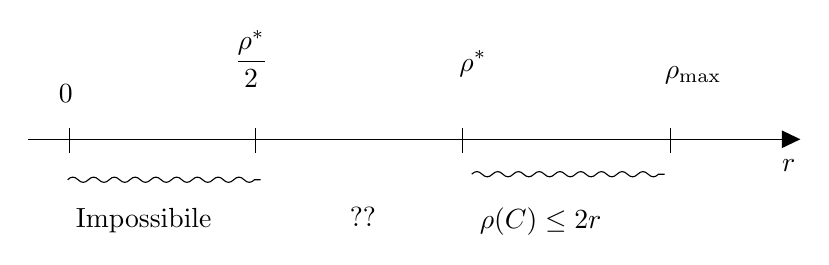
\begin{tikzpicture}[x=0.75pt,y=0.75pt,yscale=-1,xscale=1]
	\draw    (121,120.5) -- (490,120.5) ;
	\draw [shift={(493,120.5)}, rotate = 180] [fill={rgb, 255:red, 0; green, 0; blue, 0 }  ][line width=0.08]  [draw opacity=0] (8.93,-4.29) -- (0,0) -- (8.93,4.29) -- cycle    ;
	\draw    (230.33,115) -- (230.33,127) ;
	\draw    (330.33,115) -- (330.33,127) ;
	\draw    (430.33,115) -- (430.33,127) ;
	\draw    (140.75,115) -- (140.75,127) ;
	\draw    (140,140) .. controls (141.67,138.33) and (143.33,138.33) .. (145,140) .. controls (146.67,141.67) and (148.33,141.67) .. (150,140) .. controls (151.67,138.33) and (153.33,138.33) .. (155,140) .. controls (156.67,141.67) and (158.33,141.67) .. (160,140) .. controls (161.67,138.33) and (163.33,138.33) .. (165,140) .. controls (166.67,141.67) and (168.33,141.67) .. (170,140) .. controls (171.67,138.33) and (173.33,138.33) .. (175,140) .. controls (176.67,141.67) and (178.33,141.67) .. (180,140) .. controls (181.67,138.33) and (183.33,138.33) .. (185,140) .. controls (186.67,141.67) and (188.33,141.67) .. (190,140) .. controls (191.67,138.33) and (193.33,138.33) .. (195,140) .. controls (196.67,141.67) and (198.33,141.67) .. (200,140) .. controls (201.67,138.33) and (203.33,138.33) .. (205,140) .. controls (206.67,141.67) and (208.33,141.67) .. (210,140) .. controls (211.67,138.33) and (213.33,138.33) .. (215,140) .. controls (216.67,141.67) and (218.33,141.67) .. (220,140) .. controls (221.67,138.33) and (223.33,138.33) .. (225,140) .. controls (226.67,141.67) and (228.33,141.67) .. (230,140) -- (233,140) -- (233,140) ;
	\draw    (334.67,137.33) .. controls (336.34,135.66) and (338,135.66) .. (339.67,137.33) .. controls (341.34,139) and (343,139) .. (344.67,137.33) .. controls (346.34,135.66) and (348,135.66) .. (349.67,137.33) .. controls (351.34,139) and (353,139) .. (354.67,137.33) .. controls (356.34,135.66) and (358,135.66) .. (359.67,137.33) .. controls (361.34,139) and (363,139) .. (364.67,137.33) .. controls (366.34,135.66) and (368,135.66) .. (369.67,137.33) .. controls (371.34,139) and (373,139) .. (374.67,137.33) .. controls (376.34,135.66) and (378,135.66) .. (379.67,137.33) .. controls (381.34,139) and (383,139) .. (384.67,137.33) .. controls (386.34,135.66) and (388,135.66) .. (389.67,137.33) .. controls (391.34,139) and (393,139) .. (394.67,137.33) .. controls (396.34,135.66) and (398,135.66) .. (399.67,137.33) .. controls (401.34,139) and (403,139) .. (404.67,137.33) .. controls (406.34,135.66) and (408,135.66) .. (409.67,137.33) .. controls (411.34,139) and (413,139) .. (414.67,137.33) .. controls (416.34,135.66) and (418,135.66) .. (419.67,137.33) .. controls (421.34,139) and (423,139) .. (424.67,137.33) -- (427.67,137.33) -- (427.67,137.33) ;

	\draw (483,129) node [anchor=north west][inner sep=0.75pt]   [align=left] {$\displaystyle r$};
	\draw (134.5,93) node [anchor=north west][inner sep=0.75pt]   [align=left] {$\displaystyle 0$};
	\draw (219,67) node [anchor=north west][inner sep=0.75pt]   [align=left] {$\displaystyle \frac{\rho ^{*}}{2}$};
	\draw (327.5,76.5) node [anchor=north west][inner sep=0.75pt]   [align=left] {$\displaystyle \rho ^{*}$};
	\draw (426.5,84) node [anchor=north west][inner sep=0.75pt]   [align=left] {$\displaystyle \rho_{\max}$};
	\draw (142.67,152.67) node [anchor=north west][inner sep=0.75pt]   [align=left] {Impossibile};
	\draw (337.33,152) node [anchor=north west][inner sep=0.75pt]   [align=left] {$\rho(C)\leq 2r$};
	\draw (274.67,152) node [anchor=north west][inner sep=0.75pt]   [align=left] {??};
\end{tikzpicture}

	\caption{Comportamento di \CenterSelectionPlus.}
	\label{fig:csplus_r_beh}
\end{figure}


\subsection{\GreedyCenterSelection}
L'algoritmo \ref{algo:GreedyCenterSelection} è un algoritmo greedy per \CenterSelection.

\begin{algorithm}
	\caption{\GreedyCenterSelection}
	\SetKwFunction{ExtractRandomPoint}{ExtractRandomPoint}

\KwInput{$S$, $k$, $d$}

\If{$\card S\leq k$}{
	\Return $S$\;
}
$s\asn\ExtractRandomPoint(S)$\;
$C\asn C\cup \set{s}$\;
\While{$\card C\leq k$}{
	$\bar s\asn\arg\max_{s\in S} d(s,C)$\;
	$C\asn C\cup\set{\bar s}$\;
}
\Return $C$\;

	\label{algo:GreedyCenterSelection}
\end{algorithm}

\begin{theorem}
	\GreedyCenterSelection è un algoritmo $2$-approssimante per \CenterSelection.
\end{theorem}
\begin{proof}
	Per assurdo, supponiamo che $C$ sia tale che $\rho(C)>2\rho\star$, ossi  esiste $\hat s\in S$ tale che $d(\hat s,C)> 2\rho\star$.
	Consideriamo l'$i$-esima iterazione dell'algoritmo: sia $C_i$ l'insieme dei centri all'inizio dell'$i$-esima iterazione e $\bar s_i$ il centro da inserire. Vale:
	\begin{equation*}
		d(\bar s_i,C_i)\geq d(\hat s,C_i)\geq d(\hat s, C)>2\rho\star
	\end{equation*}
	Questa condizione è esattamente quella che esclude punti dalla selezione di \CenterSelectionPlus', pertanto i due algoritmi sono equivalenti se $r=\rho\star$. Ma per $r=\rho\star$ \CenterSelectionPlus' emette una $\frac{2\rho\star}{\rho\star}=2$-approssimazione, il che contraddice l'ipotesi di assurdo.
\end{proof}

\begin{theorem}
	Se $\P\neq\NP$, non esiste $\alpha<2$ tale che $\CenterSelection\in\gAPX\alpha$.
\end{theorem}
\begin{proof}
	Si consideri il problema di decisione \NP-completo \DominatingSet. Dato un grafo non orientato $G=(V,E)$, un dominating set per $G$ è un insieme di vertici $D\subseteq V$ se e solo se ogni vertice non appartenente a $D$ ha un adiacente in $D$: $\forall x\in(V\setminus D),\exists y\in D\mid \set{x,y}\in D$.

	\pdec{\DominatingSet}
	{Grafo non orientato $G=(V,E)$, $k\in\N^+$}
	{Determinare se esiste un dominating set per $G$ di cardinalità minore o uguale a $k$}

	Data un'istanza $((V,E),k)$ di \DominatingSet, costruiamo una istanza di \CenterSelection che ha per spazio l'insieme dei vertici, per numero massimo di centri il limite di cardinalità $k$ per il dominating set e per metrica la funzione
	\begin{equation*}
		d(x,y) =
		\begin{cases}
			0 \quad & \text{se } x = y                      \\
			1 \quad & \text{se } x\neq y\land\set{x,y}\in E \\
			2 \quad & \text{altrimenti}
		\end{cases}
	\end{equation*}

	In una istanza di \CenterSelection derivata in questo modo, $\rho\star=2$ oppure $\rho\star=1$. Nel secondo caso l'insieme di centri scelti è un dominating set nell'istanza originale del problema, infatti:
	\begin{align*}
		\rho\star=1 & \coimpl\forall x\in(V\setminus D)\quad d(x,D)=1                             \\
		            & \coimpl\forall x \in (V \setminus D)\quad \exists y\in D\mid d(x,y)=1       \\
		            & \coimpl\forall x \in (V \setminus D)\quad \exists y\in D\mid \set{x,y}\in E \\
		            & \coimpl D\text{ è un dominating set}
	\end{align*}

	Per assurdo, supponiamo che esista un algoritmo $\alpha$-approssimante per \CenterSelection, con $\alpha < 2$. Eseguendo tale algoritmo su un'istanza così costruita si ottiene un output $D$ tale che:
	\begin{gather*}
		1\leq\frac{\rho(D)}{\rho\star}\leq\alpha<2 \\
		\rho\star\leq\rho(D)\leq\alpha\cdot\rho\star<2\rho\star
	\end{gather*}

	Dato che $\rho\star=1\lor\rho\star=2$, allora vale esattamente una delle seguenti proposizioni:
	\begin{equation*}
		\begin{cases}
			1\leq\rho(D)<2\quad & \text{se } \rho\star=1 \\
			2\leq\rho(D)<4\quad & \text{se } \rho\star=2
		\end{cases}
	\end{equation*}
	Quindi, eseguito l'algoritmo, se $\rho(D)<2$ allora $\rho\star=1$ e la decisione per l'istanza originale di \DominatingSet è positiva; se $\rho(D)\geq2$ allora $\rho\star=2$ e la decisione è negativa.

	Poiché l'algoritmo agisce in tempo polinomiale, allora $\DominatingSet\in\P$, il che è assurdo se $\P\neq\NP$.
\end{proof}



\section{Problema della copertura d'insiemi}
Si definisce funzione armonica la funzione $H:\N^+\to\R$ tale che
\begin{equation*}
	H(n)=\sum_{k=1}^n \frac 1k
\end{equation*}

% TODO: dimostrare in un'appendice (vedi vecchi appunti)
Vale la seguente proprietà per la funzione armonica:
\begin{theorem}
	\begin{equation*}
		\ln(n+1)\leq H(n)\leq 1+\ln(n)
	\end{equation*}
\end{theorem}

\popt{\MinSetCover}
{$S_1,S_2,\dots,S_m\subseteq U$ tali che $\cup_{i=1}^m S_i=U$ e pesi $w_1,\dots,w_m$ con $w_i \in\R^{>0}~\forall i$}
{$C\subseteq\set{S_1,\dots,S_n}$}
{Quali sono gli insiemi da scegliere per coprire tutti gli elementi di $U$ col costo minore possibile?}
{$C$ tale che $\cup_{i\in C}S_i=U$}
{$\MIN$}
{$w:=\sum_{i:S_i\in C} w_i$}


\subsection{Algoritmo greedy set cover}
\begin{algorithm}[ht]
	\caption{\GreedySetCover}
	\label{algo:greedysetcover}
	\KwInput{$S_i, U$}

$R\asn U$\;
$C\asn\emptyset$\;
\While{$R\neq\emptyset$} {
	$i=\arg\min_i \set{\frac{w_i}{\card{S_i \cap R}}}$\;
	$C\asn C\cup\set{S_i}$\;
	$R\asn R\setminus S_i$\;
}
\Return{$C$}\;

\end{algorithm}
L'algoritmo \ref{algo:greedysetcover} costruisce polinomialmente una soluzione per \MinSetCover, scegliendo a ogni iterazione il sottoinsieme di input che minimizza il rapporto tra il suo peso e il numero di elementi che esso aggiunge all'output parziale.

Ogni elemento $s\in U$ viene inserito nell'output parziale in qualche iterazione $j$ con l'aggiunta di un sottoinsieme $S_j$. Definiamo quindi
\begin{equation*}
	c_u = \frac{w_j}{\card{S_j\cap R_j}}
\end{equation*}
il costo della copertura del singolo elemento di $U$, avvenuta tramite l'aggiunta di $S_j$ durante la $j$-esima iterazione.

\begin{lemma}\label{lem:gsetcov_w_sum_c_u}
	\begin{equation*}
		w=\sum_{u\in U} c_u
	\end{equation*}
\end{lemma}
\begin{proof}
	Si noti che gli insiemi $S_j\cap R_j$, dove $S_j$ è l'insieme di input scelto al passo $j$ e $R_j$ è l'insieme degli elementi dell'universo rimasti da selezionare al passo $j$, costituiscono una partizione di $U$. Infatti, l'algoritmo termina solo dopo aver esaurito gli elementi di $U$, e ogni insieme $S_j\cap R_j$ aggiunge unicamente nuovi elementi.

	Sia $w_j$ il costo dell'insieme $S_j$ aggiunto al passo $j$. Allora
	\begin{equation*}
		w = \sum_j w_j=\sum_j\sum_{s\in S_j\cap R_j} c_s=\sum_{u\in U} c_u
	\end{equation*}
\end{proof}
\begin{lemma}\label{lem:gsetcov_cu_leq_harmoskwk}
	\begin{equation*}
		\forall k\in\set{1,\dots,m} \quad\sum_{s\in S_k} c_u\leq H(\card{S_k}) \cdot w_k
	\end{equation*}
\end{lemma}
\begin{proof}
	Sia $S_k=\set{u_1,u_2,\dots,u_d}$, dove gli elementi sono elencati in ordine di copertura.

	Quando un elemento $s_j$ viene coperto dall'inserimento di un insieme $S_{k'}$, gli elementi di $S_k$ ancora da inserire spaziano almeno da $s_j$ a $s_d$, quindi:
	\begin{equation*}
		\card{S_k\cap R}\geq d-j+1 \text.
	\end{equation*}
	Quindi
	\begin{equation*}
		c_{s_j}=\frac{w_{k'}}{\card{S_{k'}\cap R_j}}
		\leq\frac{w_k}{\card{S_k\cap R_j}}
		\leq\frac{w_k}{d-j+1} \text.
	\end{equation*}
	E, di conseguenza
	\begin{align*}
		\sum_{s\in S_k} c_s & =c_{s_1}+c_{s_2}+c_{s_3}\dots+c_{s_d}                            \\
		                    & \leq \frac{w_k}{d-1+1}+\frac{w_k}{d-2+1}+\dots+\frac{w_k}{d-d+1} \\
		                    & \leq \frac{w_k}{d}+\frac{w_k}{d-1}+\dots+\frac{w_k}{1}           \\
		                    & = w_k\left(1 + \frac{1}{2} + \dots + \frac{1}{d}\right)          \\
		                    & = w_k\cdot H(\card{S_k})
	\end{align*}
\end{proof}

\begin{theorem}
	Sia $M=\max_i\card{S_i}$. \GreedySetCover è $H(M)$-approssimante per \MinSetCover.
\end{theorem}
\begin{proof}
	Sia $w\star:=\sum_{i:S_i\in C\star} w_i$.
	Applicato l'algoritmo, in virtù del lemma \ref{lem:gsetcov_cu_leq_harmoskwk} vale, per qualunque $i$:
	\begin{equation*}
		w_i\geq\frac{\sum_{s\in S_i} c_s}{H(\card{S_i})}\geq\frac{\sum_{s\in S_i} c_s}{H(M)}
	\end{equation*}
	Essendo $C\star$ una copertura e applicando il lemma \ref{lem:gsetcov_w_sum_c_u}:
	\begin{equation*}
		\sum_{S_i\in C\star}\sum_{s\in S_i} c_s \geq \sum_{s\in U} c_s = w
	\end{equation*}
	Applicando queste due osservazioni:
	\begin{gather*}
		w\star = \sum_{i:S_i\in C\star} w_i \geq \sum_{i:S_i\in C\star} \frac{\sum_{s\in S_i} c_s}{H(M)} \geq \frac{w}{H(M)} \\
		\frac{w}{w\star} \leq H(M)
	\end{gather*}
\end{proof}

Inoltre vale:
\begin{equation*}
	H(M)\leq H(\card U) = O(\ln(\card U))
\end{equation*}
Ergo:
\begin{corollario}
	\GreedySetCover è un algoritmo $O(\ln(n))$-approssimante per \MinSetCover, dove $n$ è la cardinalità dell'insieme universo.
\end{corollario}

Per quanto riguarda l'ottimalità di questo bound:
\begin{theorem}
	Per ogni $\varepsilon>0$, \GreedySetCover non è $(O(\ln(n))-\varepsilon)$-approssimante per \MinSetCover.
\end{theorem}
\begin{proof}
	% TODO: adattare a n non potenza di 2?
	Fissati $\varepsilon$ e $n$ (sia per semplicità $n=2^k$ per qualche $k\in\N^+,k>2$), si consideri l'input per \MinSetCover mostrato in figura \ref{fig:setcover_tightness}.
	L'input è costituito da due insiemi disgiunti $A$ e $B$ di costo $1+\varepsilon$ e cardinalità $n/2$; e $\log_2 n$ insiemi disgiunti $S_1,S_2,\dots,S_{\log_2 n}$, di cardinalità rispettive $n/2,n/4,\dots$ e costo $1$. In ciascun insieme $S_i$, metà degli elementi è contenuta in $A$ e l'altra metà in $B$.

	\begin{figure}[ht]
		\centering
		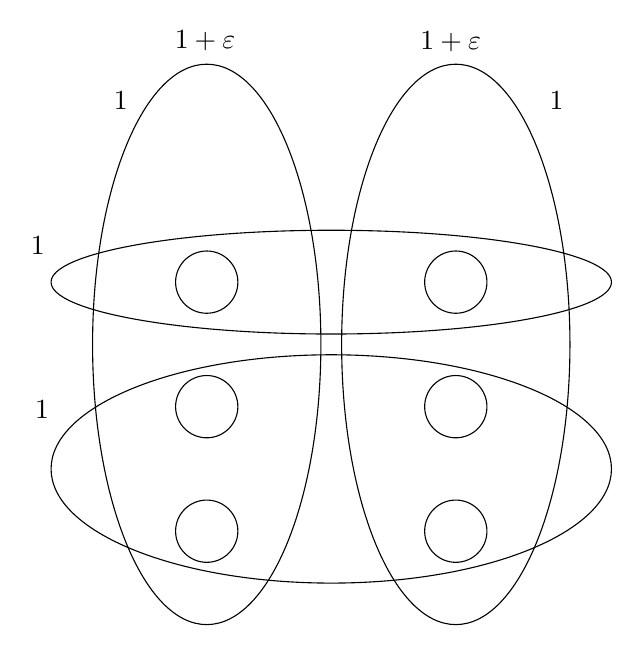
\begin{tikzpicture}[x=0.75pt,y=0.75pt,yscale=-1,xscale=1]
	\draw   (150,155) .. controls (150,80.44) and (174.62,20) .. (205,20) .. controls (235.38,20) and (260,80.44) .. (260,155) .. controls (260,229.56) and (235.38,290) .. (205,290) .. controls (174.62,290) and (150,229.56) .. (150,155) -- cycle ;
	\draw   (190,245) .. controls (190,236.72) and (196.72,230) .. (205,230) .. controls (213.28,230) and (220,236.72) .. (220,245) .. controls (220,253.28) and (213.28,260) .. (205,260) .. controls (196.72,260) and (190,253.28) .. (190,245) -- cycle ;
	\draw   (190,185) .. controls (190,176.72) and (196.72,170) .. (205,170) .. controls (213.28,170) and (220,176.72) .. (220,185) .. controls (220,193.28) and (213.28,200) .. (205,200) .. controls (196.72,200) and (190,193.28) .. (190,185) -- cycle ;
	\draw   (190,125) .. controls (190,116.72) and (196.72,110) .. (205,110) .. controls (213.28,110) and (220,116.72) .. (220,125) .. controls (220,133.28) and (213.28,140) .. (205,140) .. controls (196.72,140) and (190,133.28) .. (190,125) -- cycle ;
	\draw   (270,155) .. controls (270,80.44) and (294.62,20) .. (325,20) .. controls (355.38,20) and (380,80.44) .. (380,155) .. controls (380,229.56) and (355.38,290) .. (325,290) .. controls (294.62,290) and (270,229.56) .. (270,155) -- cycle ;
	\draw   (310,245) .. controls (310,236.72) and (316.72,230) .. (325,230) .. controls (333.28,230) and (340,236.72) .. (340,245) .. controls (340,253.28) and (333.28,260) .. (325,260) .. controls (316.72,260) and (310,253.28) .. (310,245) -- cycle ;
	\draw   (310,185) .. controls (310,176.72) and (316.72,170) .. (325,170) .. controls (333.28,170) and (340,176.72) .. (340,185) .. controls (340,193.28) and (333.28,200) .. (325,200) .. controls (316.72,200) and (310,193.28) .. (310,185) -- cycle ;
	\draw   (310,125) .. controls (310,116.72) and (316.72,110) .. (325,110) .. controls (333.28,110) and (340,116.72) .. (340,125) .. controls (340,133.28) and (333.28,140) .. (325,140) .. controls (316.72,140) and (310,133.28) .. (310,125) -- cycle ;
	\draw   (130,215) .. controls (130,184.62) and (190.44,160) .. (265,160) .. controls (339.56,160) and (400,184.62) .. (400,215) .. controls (400,245.38) and (339.56,270) .. (265,270) .. controls (190.44,270) and (130,245.38) .. (130,215) -- cycle ;
	\draw   (130,125) .. controls (130,111.19) and (190.44,100) .. (265,100) .. controls (339.56,100) and (400,111.19) .. (400,125) .. controls (400,138.81) and (339.56,150) .. (265,150) .. controls (190.44,150) and (130,138.81) .. (130,125) -- cycle ;

	\draw (119,102) node [anchor=north west][inner sep=0.75pt]   [align=left] {$1$};
	\draw (121,181) node [anchor=north west][inner sep=0.75pt]   [align=left] {$1$};
	\draw (159,32) node [anchor=north west][inner sep=0.75pt]   [align=left] {$1$};
	\draw (369,32) node [anchor=north west][inner sep=0.75pt]   [align=left] {$1$};
	\draw (188.33,2.67) node [anchor=north west][inner sep=0.75pt]   [align=left] {$1 + \varepsilon$};
	\draw (306.67,3) node [anchor=north west][inner sep=0.75pt]   [align=left] {$1 + \varepsilon$};
\end{tikzpicture}

		\caption{Esempio di input "cattivo" per $n=8$}
		\label{fig:setcover_tightness}
	\end{figure}

	L'algoritmo sceglie nell'ordine gli insiemi $S_i$ in quanto il costo di aggiungerli è, per ogni iterazione $j$, $\frac{1}{n/2^j}$, contro un costo di $\frac{1+\varepsilon}{n/2^j}$ per scegliere $A$ o $B$.
	Questo porta un costo complessivo di $\log_2 n$. La soluzione ottima tuttavia è naturalmente quella composta dagli insiemi $A$ e $B$, che ha un costo di $2+2\varepsilon$. Il rapporto tra le due è necessariamente logaritmico.
\end{proof}



\section{\VertexCover}
Una copertura per un grafo non orientato $G=(V,E)$ è un insieme di vertici $X\subseteq V$ tale che ogni lato di $E$ incide su un vertice in $X$.
Il problema \VertexCover associa a ogni vertice un peso e cerca la copertura di costo complessivo minimo.

\popt{\VertexCover}
{Grafo non orientato $G=(V,E)$ e pesi $w_1,\dots,w_n$, con $n=\card V$ e $w_i\in\Q^+~\forall i$}
{$X\subseteq V$}
{Determinare una copertura di $G$ di costo minimo}
{$X\subseteq V$ tale che $\forall e\in E ~ e\cap X\neq\emptyset$}
{$\MIN$}
{$w=\sum_{i\in X} w_i$}

Si considerino i problemi di decisione associati a \VertexCover e \MinSetCover.
Un'istanza $\tuple{G=(V,E),\angle{w_i}_{i\in V}}$ di \VertexCover può essere convertita in tempo polinomiale in una di \MinSetCover scegliendo come insiemi gli insiemi dei lati incidenti su ogni vertice $i$:
\begin{equation*}
	S_i=\set{e\in E\mid i\in e}
\end{equation*}
L'insieme universo è $E$ e i pesi sono quelli del vertice relativo a ogni insieme.

\begin{theorem}
	Sia $D$ il grado massimo di un grafo di input a \VertexCover. \VertexCover è $H(D)$-approssimabile.
\end{theorem}


\subsection{\PricedVertexCover}
Si consideri un'istanza di \VertexCover formata dal grafo $G=(V,E)$ e i pesi $\angle{w_i}_{i\in V}$.
$\angle{P_e}_{e\in E}$ è un \emph{assegnamento di prezzi} sui lati.
Un assegnamento $\angle{P_e}_{e\in E}$ si dice \emph{equo} se e solo se
\begin{equation*}
	\forall i\in V\quad\sum_{e\ni i} P_e\leq w_i \text.
\end{equation*}
Un assegnamento si dice \emph{stretto} su un vertice $i$ se e solo se
\begin{equation*}
	\sum_{e\ni i} P_e = w_i \text.
\end{equation*}

\begin{lemma}\label{lem:vcov_pricing_eq_sum_p_e_w_opt}
	Se $\angle{P_e}_{e\in E}$ è equo allora
	\begin{equation*}
		\sum_{e\in E} P_e \leq w\star
	\end{equation*}
	dove $w\star$ il costo ottimo per l'istanza di \VertexCover.
\end{lemma}
\begin{proof}
	Sia $X\star\subseteq V$ una soluzione ottima. Poiché $\angle{P_e}_{e\in E}$ è equo:
	\begin{equation*}
		\sum_{i\in X\star} \sum_{e\ni i} P_e \leq \sum_{i\in X\star} w_i = w\star
	\end{equation*}
	Ogni lato del grafo incide su un vertice di $X\star$, quindi
	\begin{equation*}
		\sum_{e\in E} P_e \leq \sum_{i\in X\star} \sum_{e\ni i} P_e \leq w\star
	\end{equation*}
\end{proof}

L'algoritmo \ref{algo:PricedVertexCover} usa una tecnica di pricing per costruire una soluzione per \VertexCover.
\begin{algorithm}
	\caption{\PricedVertexCover}
	\label{algo:PricedVertexCover}
	\KwInput{$G=(V,E)$, $\angle{w_i}_{i\in V}$}

\For{$e \in E$}{
	$P_e \asn 0$\;
}
\While{esiste un lato $\bar e=\set{\bar i,\bar j}$ tale che $\angle{P_{\bar e}}$ non è stretto né su $\bar i$ né su $\bar j$}{
	$\Delta \asn \min\set{w_{\bar i}-\sum_{e\ni\bar i} P_e , w_{\bar j}-\sum_{e\ni\bar j} P_e}$\;
	$P_{\bar e} \asn P_{\bar e} + \Delta$\;
}
$S \asn \set{v\in V \mid \angle{P_e} \text{ è stretto su } v}$\;
\Return {$S$}\;

\end{algorithm}

\begin{lemma}\label{lem:pvcov_w_le_w_sum_P_e}
	Al termine dell'esecuzione dell'algoritmo \ref{algo:PricedVertexCover} vale
	\begin{equation*}
		w \leq 2 \sum_{e \in E} P_e
	\end{equation*}
\end{lemma}
\begin{proof}
	All'uscita dal ciclo, non esistono lati $\set{i,j}$ tali che $\angle{P_e}$ non è stretto né su $i$ né su $j$.
	Quindi l'insieme $S$ dei vertici su cui $\angle{P_e}$ è stretto è una copertura.

	Essendo $S$ una soluzione ammissibile, per definizione:
	\begin{equation*}
		w = \sum_{i\in S} w_i \text.
	\end{equation*}
	Poiché $S$ contiene solo vertici su cui $\angle{P_e}$ è stretto:
	\begin{equation*}
		\forall i\in S \quad w_i = \sum_{e\ni i} P_e \text.
	\end{equation*}
	Ergo
	\begin{equation*}
		w = \sum_{i\in S} \sum_{e\ni i} P_e
	\end{equation*}
	Poiché un lato compare nella somma al più $2$ volte:
	\begin{equation*}
		w \leq 2 \sum_{e\in E} P_e
	\end{equation*}
\end{proof}

\begin{theorem}
	\PricedVertexCover è un algoritmo $2$-approssimante per \VertexCover.
\end{theorem}
\begin{proof}
	\begin{equation*}
		\frac{w}{w\star} \underset{\text{lemma \ref{lem:pvcov_w_le_w_sum_P_e}}}{\leq}
		\frac{2\sum_{e\in E} P_e}{w\star} \underset{\text{lemma \ref{lem:vcov_pricing_eq_sum_p_e_w_opt}}}{\leq}
		\frac{2\sum_{e\in E} P_e}{\sum_{e\in E} P_e} = 2
	\end{equation*}
\end{proof}


\subsection{\VertexCover tramite arrotondamento di \LinearProgramming}
Si consideri il problema di programmazione lineare e la sua versione vincolata all'integrità della soluzione, il problema di programmazione lineare intera.

\popt{\LinearProgramming}
{Sistema $Ax\geq b$, con $A\in\Q^{m\times n},b\in\Q^m$ ($x$ incognito), vettore $c\in\Q^n$.}
{Assegnamenti per $x$ in $\Q^n$}
{Determinare il vettore $x$ che minimizza la funzione obiettivo}
{$x\in\Q^n\mid Ax\geq b$}
{$\MIN$}
{Funzione obiettivo $c\trans x$}

\popt{\IntegerLinearProgramming}
{Sistema $Ax\geq b$, con $A\in\Q^{m\times n},b\in\Q^m$ ($x$ incognito), vettore $c\in\Q^n$.}
{Assegnamenti per $x$ in $\Z^n$}
{Determinare il vettore $x$ che minimizza la funzione obiettivo}
{$x\in\Z^n\mid Ax\geq b$}
{$\MIN$}
{Funzione obiettivo $c\trans x$}

Per lo stesso input, una soluzione ottima di \IntegerLinearProgramming è ammissibile, ma non necessariamente ottima, per \LinearProgramming.
Viceversa una soluzione ottima per \LinearProgramming può non essere ammissibile per un'istanza di \IntegerLinearProgramming dallo stesso input.

% TODO: cite karmakar, 1981
\LinearProgramming è un problema appartenente a \PO (l'ottimo può essere trovato polinomialmente ad esempio con l'algoritmo di Karmakar), mentre \IntegerLinearProgramming è \NPO-completo.

Data un'istanza di \VertexCover $\tuple{G=(V,E),\angle{w_i}_{i\in V}}$, con $n:=\card V$ e $m:=\card E$, si consideri l'istanza di \IntegerLinearProgramming in cui il sistema di input è così costruito:
\begin{equation*}
	\begin{cases}
		x_i\geq 0     & \qquad \forall i\in V         \\
		x_i\leq 1     & \qquad \forall i\in V         \\
		x_i+x_j\geq 1 & \qquad \forall \set{i,j}\in E \\
	\end{cases}
\end{equation*}
e la funzione obiettivo è
\begin{equation*}
	w = \min\sum_{i\in V} w_i x_i
\end{equation*}

Una soluzione $x$ dell'istanza di \IntegerLinearProgramming costruita si può interpretare come una soluzione di \VertexCover in cui $x_i=1\iff i\in X$.

Si consideri l'istanza di \LinearProgramming ottenuta rilassando il vincolo di integrità dell'istanza precedente.
Una soluzione ottima $x$ di tale istanza può essere calcolata in tempo polinomiale, ma non è, in generale, ammissibile per la sua versione intera.
Si consideri il vettore $r$, ottenuto dall'arrotondamento di $x$, ossia, per ciascun $i\in n$:
\begin{equation*}
	r_i:= \begin{cases}
		1 & \quad x_i\geq\frac{1}{2} \\
		0 & \quad x_i<\frac{1}{2}
	\end{cases}
\end{equation*}

\begin{lemma}\label{lem:ilp_r_ammiss}
	Il vettore $r$ è una soluzione ammissibile di \IntegerLinearProgramming.
\end{lemma}
\begin{proof}
	Per definizione, $0\leq r\leq 1$. Se non fosse $r_i+r_j\geq 1~\forall \set{i,j}\in E$, siano $\bar i,\bar j$ tali che $r_{\bar i}+r_{\bar j}<1$.
	Allora $r_{\bar i}=r_{\bar j}=0$. Per definizione di $r$ si ha $x_{\bar i}<\frac 12$ e $x_{\bar j}<\frac 12$.
	Ma allora $x_{\bar i}+x_{\bar j}<1$, il che contraddice l'ammissibilità di $x$.
\end{proof}

\begin{lemma}\label{lem:ilp_r_i_leq_2_x_i}
	\begin{equation*}
		\forall i\in V \qquad r_i \leq 2x_i
	\end{equation*}
\end{lemma}
\begin{proof}
	Se $r_i=0$ la disuguaglianza è ovvia;
	se $r_i=1$ allora, $x_i\geq \frac 12$ e $2x_i\geq 1=r_i$.
\end{proof}

\begin{theorem}\label{lem:ilp_appr}
	L'insieme $\set{i\in V\mid r_i=1}$ è una $2$-approssimazione per \VertexCover.
\end{theorem}
\begin{proof}
	Sia $w:=\sum{i\in V} w_i r_i$ il costo della soluzione di \VertexCover indotta dall'istanza arrotondata di \LinearProgramming, e sia $w\star$ la soluzione ottima. Si denoti con $w\star_{\text{LP}}$ il costo ottimo dell'istanza di \LinearProgramming e $w\star_{\text{ILP}}$ quello di \IntegerLinearProgramming.
	Applicando il lemma \ref{lem:ilp_r_i_leq_2_x_i}:
	\begin{equation*}
		w = \sum_{i\in V} w_i r_i \leq 2\sum_{i\in V} w_i x_i = 2w\star_{\text{LP}} \leq 2w\star_{\text{ILP}} = w\star
	\end{equation*}
\end{proof}





\section{\DisjointPaths}
Dato un grafo orientato su cui sono selezionati un numero di vertici \flang{source} e un numero di rispettivi vertici \flang{target}, il problema \DisjointPaths si pone l'obiettivo di massimizzare il numero di coppie source-target connettibili da un cammino usando ogni arco un numero massimo di $c$ volte, dove $c$ è un dato parametro. Il problema prende il nome dalla sua variante con $c=1$, in cui i cammini non hanno archi in comune.

\popt{\DisjointPaths}
{Grafo orientato $G=(V,E)$, vertici $\angle{s_i}_{i\in k}$ e $\angle{t_i}_{i\in k}$ e un parametro $c\in\N^+$}
{$I\subseteq k$, cammini $\angle{\pi_i}_{i\in I}$, con $\pi_i:=s_i\leadsto t_i$}
{Determinare il massimo numero di coppie $s_i,t_i$ che si possono connettere con un cammino, usando un arco al più $c$ volte complessivamente}
{$I\subseteq k$, cammini $\angle{\pi_i}_{i\in I}$ tali che nessun arco $e\in E$ appartenga ai cammini più di $c$ volte}
{$\MAX$}
{$\card I$}


\subsection{\PricedDisjointPaths}
L'algoritmo \ref{algo:PricedDisjointPaths} usa una tecnica di pricing in cui viene definita una funzione di costo $l:E\to\Q^+$ per gli archi, estendibile ai cammini $\tuple{x_0,x_1\dots,x_{t-1},x_t}$ con $l(\tuple{x_0,x_1,\dots,x_{t-1},x_t}):=l((x_0,x_1))+\dots+l((x_{t-1},x_t))$.
L'algoritmo fa inoltre uso di un valore $\beta$ che, come si vedrà, può essere calcolato in modo da ottimizzare il risultato.
\SetKwFunction{MinPath}{MinPath}
La procedura \MinPath restituisce, in tempo polinomiale, un cammino di costo minimo e l'indice $i$ dei vertici $s_i$ e $t_i$ che collega, con $i\notin I$. Se un cammino del genere non esiste, la procedura restituisce un cammino vuoto.
L'algoritmo produce una soluzione ammissibile per \DisjointPaths, dal momento che $P$ contiene solo cammini con archi utilizzati al più $c$ volte (dopo $c$ volte un arco viene eliminato) e che collegano, per definizione di \MinPath, vertici non ancora collegati.
\PricedDisjointPaths ha un costo polinomiale: utilizzando ad esempio Floyd-Warshall la procedura \MinPath può essere implementata in $O(\card V^3)$ e viene ripetuta un massimo di $k$ volte, per un costo totale in tempo di $O(k\card V^3)$.

\begin{algorithm}
	\caption{\PricedDisjointPaths}
	\label{algo:PricedDisjointPaths}
	\KwInput{$G=(V,E), \angle{s_i}_{i\in k}, \angle{t_i}_{i\in k}, c\in\N^+, b\in\Q^+$}

$I \asn \emptyset$\;
$P \asn \emptyset$\;
\For{$e\in E$}{
	$l(e) \asn 1$\;
}
\While{true}{
	$\pi,i \asn \MinPath(G,l)$\;
	\If{$\pi=\langle\rangle$}{
		\Return{$I,P$}\;
	}
	$I \asn I\cup\set{i}$\;
	$P \asn P\cup\set{\pi}$\;

	\tcc{Aggiorna i costi ed elimina gli archi già usati $c$ volte}
	\For{$e\in\pi$}{
		$l(e) = l(e) \cdot \beta $\;
		\If{$l(e) = \beta^c$}{
			elimina $e$ \;
		}
	}
}


\end{algorithm}

A una data iterazione dell'algoritmo, un cammino $\pi$ si dice \emph{corto} se e solo se $l(\pi)<\beta^c$.
Un cammino $\pi$ si dice \emph{utile} se e solo se collega una coppia $i\notin I$.

Finché esistono cammini corti e utili, l'algoritmo seleziona uno di essi a ogni iterazione.
Quando nessun cammino corto è utile, l'esecuzione si ferma oppure iniziano a venire selezionati cammini lunghi.
Si consideri la prima iterazione $\bar t$ in cui non esistono cammini corti e utili, o il termine dell'esecuzione se tale iterazione non esiste.
Sia $\bar l$ la funzione di costo in tale iterazione e $\bar I$ l'insieme degli indici dei vertici collegati da cammini.

\begin{lemma}\label{lem:priceddpaths_non_included_non_short}
	Se all'iterazione $\bar t$ la coppia $\tuple{s_i,t_i}$ non è stata collegata dalla soluzione corrente, allora il costo del relativo cammino ottimo è maggiore o uguale a $\beta^c$:
	\begin{equation*}
		\bar l(\pi\star_i)\geq\beta^c\qquad\forall i\notin I
	\end{equation*}
\end{lemma}
\begin{proof}
	Se fosse $\bar l(\pi\star_i)<\beta^c$, allora $\pi\star$ sarebbe corto e utile, pertanto sarebbe stato selezionato prima dell'iterazione $\bar t$.
\end{proof}

\begin{lemma}\label{lem:priceddpaths_sum_l_a_leq_bc_i_m}
	Sia $m:=\card E$.
	\begin{equation*}
		\sum_{e\in E}\bar l(e) \leq \beta^{c+1}\card{\bar I} + m
	\end{equation*}
\end{lemma}
\begin{proof}~
	\begin{itemize}
		\item Alla prima iterazione, $\sum_{e\in E} l_0(e) = \sum_{e\in E} 1 = m$.
		\item Al termine di ogni iterazione $j<\bar t$, si modificano i valori $l_j$ in valori $l_{j+1}$ così scelti:
		      \begin{equation*}
			      l_{j+1}(e) =
			      \begin{cases}
				      l_j(e)            & \quad\text{se } e\notin\pi_i \\
				      \beta\cdot l_j(e) & \quad\text{se } e\in\pi_i
			      \end{cases}
		      \end{equation*}
		      Si consideri la differenza tra i pesi complessivi all'iterazione $j$ e quelli all'iterazione $j+1$:
		      \begin{align*}
			      \sum_{e\in E} l_{j+1}(e) - \sum_{e\in E} l_j(e) & = \sum_{e\in E} (l_{j+1}(e)-l_j(e))   \\
			                                                      & = \sum_{e\in\pi}(\beta l_j(e)-l_j(e)) \\
			                                                      & = \sum_{e\in\pi} (\beta-1)l_j(e)      \\
			                                                      & \leq \beta\sum_{e\in\pi}l_j(e)
		      \end{align*}
		      Tale valore è al più uguale a $\beta^{c+1}$, essendo il cammino $\pi$ corto perché $j<\bar t$.
	\end{itemize}
	Quindi, all'inizio dell'iterazione $\bar t$, a un costo iniziale di $m$ sono state aggiunte $\card{\bar I}$ variazioni (una per ogni iterazione e quindi aggiunta di cammini a $I$) di al più $\beta^c$ l'una, ergo:
	\begin{equation*}
		\sum_{e\in E} \bar l(e) \leq \beta^{c+1}\card{\bar I}+m \text.
	\end{equation*}
\end{proof}

\begin{corollario}\label{cor:priceddpaths_cor_1}
	\begin{equation*}
		\sum_{i\in I\star\setminus I} \bar l(\pi_i\star) \geq \beta^c \card{I\star\setminus I} \text.
	\end{equation*}
\end{corollario}
\begin{proof}
	Ottenuto dal lemma \ref{lem:priceddpaths_non_included_non_short} sommando per i valori in $I\star\setminus I$.
\end{proof}

\begin{corollario}\label{cor:priceddpaths_cor_2}
	\begin{equation*}
		\sum_{i\in I\star\setminus I} \bar l(\pi\star_i) \leq c(\beta^{c+1}\card{\bar I}+m) \text.
	\end{equation*}
\end{corollario}
\begin{proof}
	\begin{align*}
		\sum_{i\in I\star\setminus I} \bar l(\pi\star_i) & \leq \sum_{i\in I\star} \bar l(\pi\star_i)                                                                                     \\
		                                                 & \leq c \sum_{e\in E} \bar l(e)             &  & \text{ogni arco è usato al più $c$ volte nella soluzione ammissibile $I\star$} \\
		                                                 & \leq c (\beta^{c+1}\card{\bar I}+m)        &  & \text{dal lemma \ref{lem:priceddpaths_sum_l_a_leq_bc_i_m}}
	\end{align*}
\end{proof}

\begin{theorem}\label{thm:priceddpaths_approx}
	\PricedDisjointPaths è un algoritmo $1+c(\beta+\beta^{-c}m)$-approssimante per \DisjointPaths.
	Se $\beta=m^{\frac{1}{c+1}}$, \PricedDisjointPaths fornisce una $(1+2cm^{\frac{1}{c+1}})$-approssimazione.
\end{theorem}
\begin{proof}
	Sia $I\star$ la soluzione ottima e $I$ la soluzione prodotta da \PricedDisjointPaths.
	\begin{align*}
		\beta^c\card{I\star} & = \beta^c\card{I\star\cap I}+\beta^c\card{I\star\setminus I}                                                                                  \\
		                     & \leq \beta^c\card{I\star\cap I} + \sum_{i\in I\star\setminus I} \bar l(\pi\star_i) &  & \text{per il corollario \ref{cor:priceddpaths_cor_1}} \\
		                     & \leq \beta^c\card I + \sum_{i\in I\star\setminus I} \bar l(\pi\star_i)                                                                        \\
		                     & \leq \beta^c\card I + c(\beta^{c+1}\card{\bar I}+m)                                &  & \text{per il corollario \ref{cor:priceddpaths_cor_2}} \\
		                     & \leq \beta^c\card I + c(\beta^{c+1}\card I+m)                                      &  & \text{essendo $\bar I\subseteq I$} \text.
	\end{align*}
	Dividendo per $\beta^c$:
	\begin{align*}
		\card{I\star} & \leq \card I+c\beta\card I+c\beta^{-c}m                                                   \\
		              & \leq \card I+c\beta\card I+c\beta^{-c}m\card I &  & \text{essendo $\card I\geq 1$} \text.
	\end{align*}
	Dividendo per $\card I$:
	\begin{equation*}
		\frac{\card{I^*}}{\card I} \leq 1+c\beta+c\beta^{-c}m = 1+c(\beta+\beta^{-c}m)
	\end{equation*}
	% TODO: dimostrare in un'appendice
	Questo valore è minimizzato per $\beta=m^{\frac{1}{c+1}}$, ottenendo:
	\begin{align*}
		\frac{\card{I^*}}{\card I} & \leq 1+c\left(m^{\frac{1}{c+1}}+m^{\frac{-c}{c+1}}m\right) \\
		                           & = 1+c\left(m^{\frac{1}{c+1}}+m^{\frac{-c+c+1}{c+1}}\right) \\
		                           & = 1+2cm^{\frac{1}{c+1}}
	\end{align*}
\end{proof}

In effetti, l'analisi dimostra che le sole prime $\bar t$ iterazioni producono una $(1+2cm^{\frac{1}{c+1}})$-approssimazione. Dal momento che, come mostrato nella dimostrazione, $\bar I\subseteq I$, l'algoritmo al termine dell'esecuzione produce una soluzione quantomeno non peggiore.



\section{\TravelingSalesman}
Il problema del commesso viaggiatore, o \TravelingSalesman (problem, abbreviato in TSP), è uno dei problemi più famosi della teoria dei grafi.
Il problema consiste nel trovare un circuito hamiltoniano di costo minimo in un grafo pesato sugli archi.
Dato un grafo non orientato, un \emph{circuito hamiltoniano} è un circuito che passa per ogni vertice del grafo una e una sola volta.

\popt{\TravelingSalesman}
{Grafo non orientato $G=(V,E)$, pesi $\angle{\delta_e}_{e\in E}$}
{$\pi\subseteq E$ ordinato}
{Determinare il circuito hamiltoniano di minor costo}
{$\pi$ forma un circuito hamiltoniano}
{$\MIN$}
{$\sum_{e\in\pi} \delta_e$}

Con un abuso di notazione useremo $\delta$ per indicare il costo del suo argomento, inteso come la somma dei pesi degli archi che lo compongono.

L'algoritmo di Christofides, che descriveremo a breve, mette insieme una serie di risultati, problemi e algoritmi e trova un'approssimazione della soluzione ottima di \TravelingSalesman. Introduciamo ora tali nozioni.


\subsection{Requisiti}

\subsubsection{Circuiti euleriani}
Dato un grafo non orientato, un \emph{circuito euleriano} è un circuito che include ogni lato del grafo una e una sola volta. Si noti che possono esistere circuiti euleriani che includono un vertice multiple volte.

Il problema di trovare un circuito euleriano in un grafo (o multigrafo) è stato formalizzato da Eulero a partire dal problema dei ponti di Könisberg, che chiedeva se fosse possibile attraversare tutti i ponti della città una volta e tornare al punto di partenza.
Eulero dimostra una condizione necessaria e sufficiente per l'esistenza di un cammino euleriano in un multigrafo:
\begin{theorem}[di Eulero]\label{thm:eulero}
	Un multigrafo ammette un circuito euleriano se e solo se è connesso e tutti i suoi vertici hanno grado pari.
\end{theorem}

Un risultato fondamentale inerente alla parità del grado dei vertici è il lemma delle strette di mano (\flang{handshaking lemma}):
\begin{lemma}[delle strette di mano]\label{lem:handshaking}
	In ogni grafo, il numero di vertici di grado dispari è pari.
\end{lemma}
\begin{proof}
	Dal momento che ogni arco aumenta il grado di due vertici, la somma dei gradi di tutti i vertici è pari. Ma una somma di interi è pari se e solo se il numero di addendi dispari è pari.
\end{proof}

\subsubsection{Il TSP metrico su cricca}\label{subsub:tsp:criccametrica}

\paragraph{Il TSP su cricca} A partire da un'istanza di \TravelingSalesman composta dal grafo $G=(V,E)$ e i pesi $\angle{\delta_e}_{e\in E}$, si consideri l'istanza composta dalla cricca $K=\left(V,\binom V 2\right)$ e dai pesi $\angle{\bar\delta}_{e\in\binom V 2}$ così definiti:
\begin{equation*}
	\bar\delta_e = \begin{cases}
		\delta_e                 & \quad e \in E    \\
		1+\sum_{e\in E} \delta_e & \quad e \notin E
	\end{cases}
\end{equation*}
Trovando la soluzione ottima di \TravelingSalesman su questa istanza, è facile determinare se il circuito hamiltoniano trovato è una soluzione per il grafo originale.
Poiché ogni arco viene percorso al più una volta (altrimenti i vertici verrebbero ripetuti nel circuito), se il costo totale è al più $\sum_{e\in E} \delta_e$ allora nessun arco assente nel grafo originale è stato usato, e la soluzione è ottima anche per l'istanza originale.
Viceversa, se il costo totale è almeno $1+\sum_{e\in E} \delta_e$ allora non è stato possibile trovare un circuito euleriano che non usasse un arco assente nell'istanza originale, e quindi questa non ha soluzione.
Si può semplificare la risoluzione di \TravelingSalesman limitandosi a risolvere il problema nel caso di cricche.

\paragraph{Il TSP metrico} Semplifichiamo ora il problema, imponendo una caratteristica "metrica" alla funzione dei pesi, cioè la disuguaglianza triangolare:
\begin{equation*}
	\delta_{\set{i,j}} \leq \delta_{\set{i,k}} + \delta_{\set{k,j}}
\end{equation*}
Come vedremo, solo grazie a questa assunzione è possibile costruire algoritmi approssimanti per \TravelingSalesman.

\subsubsection{L'albero ricoprente minimo}
Dato un grafo non orientato connesso, un albero ricoprente è un sottografo che sia un albero e mantenga tutti i vertici.
Se il grafo è pesato sui lati, un albero ricoprente minimo è quello che minimizza la somma dei costi dei lati che mantiene.
\MinimumSpanningTree (MST) è il problema di ottimizzazione che cerca l'albero ricoprente minimo.
Il problema è risolvibile esattamente in tempo polinomiale, ad esempio dall'algoritmo di Kruskal in tempo $O(m\log n)$.

\popt{\MinimumSpanningTree}
{Grafo connesso $G=(V,E)$, pesi $\angle{\delta_e}_{e\in E}$}
{Albero $T=(V',E')$}
{Trovare un albero ricoprente minimo per $G$}
{$T$ è un albero tale che $V'=V$}
{$\MIN$}
{$\sum_{e\in E'} \delta_e$}

\subsubsection{\MinimumWeightPerfectMatching}
Dato un grafo non orientato con un numero pari di vertici, un \emph{matching perfetto} è un matching (vedi \ref{sec:BiMaxMatching}) che coinvolge tutti i vertici.
In un grafo pesato sugli archi, \MinimumWeightPerfectMatching è il problema di trovare il matching perfetto a costo complessivo minimo.
\MinimumWeightPerfectMatching è risolvibile esattamente in tempo polinomiale, ad esempio con il \flang{blooming algorithm} in tempo $O(m\log n)$.

\popt{\MinimumWeightPerfectMatching}
{Grafo $G=(V,E)$ tale che $\card V$ è pari, pesi $\angle{\delta_e}_{e\in E}$}
{Matching $M\subseteq E$}
{Determinare un matching perfetto di costo minimo}
{$M$ è un matching perfetto su $G$}
{$Min$}
{$\sum_{e\in M} \delta_e$}


\subsection{L'algoritmo di Christofides}
L'algoritmo di Christofides per TSP metrico su cricca applica i concetti precedentemente descritti manipolando diverse strutture fino a ottenere un cammino hamiltoniano. Ricevendo in input una cricca $G=(V,E)$ e pesi $\angle{\delta_e}_{e\in E}$, i passi dell'algoritmo sono i seguenti:
\begin{enumerate}
	\item identificare un albero ricoprente minimo $T$ per $G$;
	\item sia $D$ il grafo indotto su $G$ dall'insieme dei suoi vertici che hanno grado dispari in $T$.
	      Questi sono in numero pari per il lemma \ref{lem:handshaking}. È quindi possibile identificare un matching perfetto minimo $M$ su $D$;
	\item sia $H$ il multigrafo indotto su $G$ dall'unione disgiunta dei lati di $T$ ed $M$. In $H$ tutti i vertici hanno grado pari, poiché quelli che avevano grado dispari in $T$ hanno un nuovo arco grazie a $M$. In virtù del lemma \ref{thm:eulero} si può trovare un circuito euleriano $\pi$ in $H$;
	\item trasformare il circuito euleriano $\pi$, valido anche per $G$, in un hamiltoniano $\tilde\pi$.
	      Ogni volta che $\pi$ passa su un vertice $v$ una seconda volta tramite i lati $\set{a,v}$ e $\set{v,b}$, è sufficiente "saltare" tale vertice sostituendo in $\tilde\pi$ i due lati con il lato $\set{a,b}$ (esistente in quanto si sta lavorando sulla cricca originale), con conseguente diminuzione del costo in virtù della disuguaglianza triangolare.
\end{enumerate}

L'analisi dell'algoritmo ci porta a dimostrare un risultato di approssimazione rispetto al TSP metrico su cricca.
\begin{lemma}\label{lem:chri_spanning}
	In una cricca $G$ pesata metricamente sui lati, il costo $\delta(T)$ dell'albero ricoprente minimo $T$ non è peggiore del costo minimo $\delta\star$ di un cammino hamiltoniano su $G$:
	\begin{equation*}
		\delta(T) \leq \delta\star
	\end{equation*}
\end{lemma}
\begin{proof}
	Sia $\pi\star$ un circuito hamiltoniano ottimo e sia $e\in\pi\star$.
	Il grafo indotto da $\pi\star\setminus e$ è un albero ricoprente. Pertanto:
	\begin{equation*}
		\delta(T) \leq \delta(\pi\star\setminus e) \leq\delta\star \text.
	\end{equation*}
\end{proof}

\begin{lemma}\label{lem:chri_matching}
	\begin{equation*}
		\delta(M) \leq \frac 1 2 \delta\star
	\end{equation*}
\end{lemma}

\begin{theorem}
	L'algoritmo di Christofides è $\frac 3 2$-approssimante per il TSP metrico su cricca.
\end{theorem}
\begin{proof}
	Per la costruzione del circuito hamiltoniano $\tilde\pi$ a partire dal circuito euleriano $\pi$ e grazie ai lemmi sopra dimostrati:
	\begin{equation*}
		\delta(\tilde\pi)\leq\delta(\pi) = \delta(T)+\delta(M)\leq
		\underbrace{\delta\star}_{\text{lemma \ref{lem:chri_matching}}} + \underbrace{\frac{\delta\star}{2}}_{\text{lemma \ref{lem:chri_spanning}}} =
		\frac 3 2 \delta\star \text.
	\end{equation*}
\end{proof}

\begin{theorem}
	Per ogni $\varepsilon>0$ esiste un input del TSP metrico su cricca su cui l'algoritmo di Christofides produce una soluzione $\pi$ tale che
	\begin{equation*}
		\frac 3 2-\varepsilon \leq \frac{\delta(\pi)}{\delta\star}
	\end{equation*}
\end{theorem}
\begin{proof}
	Dato $n$ pari e $\epsilon\in(0,1)$, si consideri il grafo in figura \ref{fig:christotight}, in cui gli archi sono etichettati con i loro pesi. Si estenda il grafo a una cricca $G$, in cui ogni lato $\set{u,v}$ non rappresentato ha come peso il peso del cammino minimo tra $u$ e $v$ sul grafo originale.

	\begin{figure}[ht]
		\centering
		\begin{tikzpicture}
	\node[minimum size=15pt, draw, circle] (1) {$v_1$};
	\node[minimum size=15pt, draw, circle, right =of 1] (2) {$v_2$};
	\node[minimum size=15pt, draw, circle, right =of 2] (3) {$v_3$};
	\node[minimum size=15pt, draw, circle, right =of 3] (4) {$v_4$};
	\node[minimum size=15pt, draw, circle, right =of 4] (5) {$v_{n-2}$};
	\node[minimum size=15pt, draw, circle, right =of 5] (6) {$v_{n-1}$};
	\node[minimum size=15pt, draw, circle, right =of 6] (7) {$v_{n}$};

	\draw[] (1) to node [auto] {$1$} (2);
	\draw[bend right=35] (1) to node [below] {$1 + \epsilon$} (3);
	\draw[] (2) to node [auto] {$1$} (3);
	\draw[bend left=35] (2) to node [auto] {$1+\epsilon$} (4);
	\draw[] (3) to node [auto] {$1$} (4);
	\draw[bend right=30] (3) edge node [below] {$1 + \epsilon$}(5.5,-1);
	\draw[dotted] (4) to (5);
	\draw[] (5) to node [auto] {$1$} (6);
	\draw[bend left=35] (5) to node [auto] {$1+\epsilon$} (7);
	\draw[] (6) to node [auto] {$1$} (7);
	\draw[bend left=30] (6) edge node [auto] {$1 + \epsilon$} (7.5,-1);
\end{tikzpicture}

		\caption{Esempio di input "cattivo" per l'algoritmo di Christofides.}
		\label{fig:christotight}
	\end{figure}

	L'algoritmo di Christofides identifica l'albero ricoprente $T$ indotto da tutti i lati di peso $1$, quindi $\delta(T)=n-1$.
	L'algoritmo seleziona poi $D=\set{v_1,v_n}$ e su di esso il matching $M$ composto dal solo lato $\set{v_1,v_n}$ di peso $\delta(M)=(1+\varepsilon)\left(\frac n2-1\right)+1$.
	Sul grafo indotto dall'unione $H$ di $T$ e $M$ l'algoritmo costruisce il circuito euleriano, nonché hamiltoniano, composto dall'unione degli archi di peso $1$ e l'arco che compone $M$.
	Il costo $\delta$ del circuito costruito è quindi:
	\begin{equation*}
		\delta = n-1 + (1+\varepsilon)\left(\frac n2-1\right)+1 = \frac32n+\varepsilon\left(\frac n2-1\right)-1 \text.
	\end{equation*}
	Ma il circuito hamiltoniano ottimo è quello che, a partire da $v_1$, percorre tutti gli archi di peso $1+\varepsilon$ che uniscono vertici di indice dispari, l'arco $\set{v_{n-1},v_n}$, tutti gli archi di peso $1+\varepsilon$ di indice pari e infine l'arco $\set{v_1,v_2}$.
	Il costo $\delta\star$ di tale circuito è:
	\begin{equation*}
		\delta\star = 2(1+\varepsilon)\left(\frac n2-1\right) + 2 = n+\varepsilon(n-2) \text.
	\end{equation*}
	Quindi
	\begin{equation*}
		\frac{\delta}{\delta\star} = \frac{\frac32n+\varepsilon\left(\frac n2-1\right)-1}{n+\varepsilon(n-2)} \geq \frac 3 2-\varepsilon \text.
	\end{equation*}
	Inoltre, per $n\to\infty$ e $\varepsilon\to0$:
	\begin{equation*}
		\frac{\delta}{\delta\star} \to \frac 3 2 \text.
	\end{equation*}
\end{proof}


\subsection{Inapprossimabilità di \TravelingSalesman}
Abbandonando l'ipotesi di disuguaglianza triangolare della funzione $\delta$, il problema \TravelingSalesman è inapprossimabile.
Al fine di dimostrare ciò ricordiamo che decidere se un grafo contiene un cammino hamiltoniano è un problema \NP-completo.

\begin{theorem}
	Se $\P\neq\NP$, non esiste alcun $\alpha>1$ tale che \TravelingSalesman sia $\alpha$-approssimabile.
\end{theorem}
\begin{proof}
	Fissato $\alpha>1$, sia $G=(V,E)$ un grafo non orientato in cui tutti i lati hanno peso $1$.
	Sia $G'$ la sua estensione a cricca, ottenuta con il metodo citato nel paragrafo \ref{subsub:tsp:criccametrica}, ossia in cui la funzione peso $\delta$ è così definita:
	\begin{equation*}
		\delta(x,y) = \begin{cases}
			1                 & \quad \set{x,y}\in E    \\
			% TODO: è davvero necessario il ceil, avendo già il +1?
			\ceil{\alpha n}+1 & \quad \set{x,y}\notin E
		\end{cases}
	\end{equation*}
	Se $G$ ammette un circuito hamiltoniano, allora tale circuito è ammesso anche in $G'$ e ha costo $n<\alpha n$.
	Viceversa, se $G$ non ammette un circuito hamiltoniano allora ogni circuito hamiltoniano in $G'$ ha costo di almeno $\ceil{\alpha n}+1$.

	Se esiste un algoritmo $\alpha$-approssimante per \TravelingSalesman, questo trova in tempo polinomiale un circuito hamiltoniano in $G'$ di costo al più $\alpha n$. Ma un tale circuito esiste se e solo se esiste un cammino hamiltoniano in $G$. L'algoritmo decide quindi in tempo polinomiale se un grafo $G$ ammette un cammino hamiltoniano, il che è impossibile se $\P\neq\NP$.
\end{proof}



% TODO: spostare insieme a LB? (se sì, sistemare l'introduzione)
\section{\texorpdfstring{$2$}{2}-\LoadBalancing}
$2$-\LoadBalancing è una specializzazione di \LoadBalancing in cui il numero di macchine $m$ è uguale a $2$.
Questo problema è anche chiamato \MinimumPartition in quanto è equivalente al bilanciare una partizione insiemistica di due elementi.

L'algoritmo \ref{algo:partitionbalance} è un algoritmo \PTAS-caratterizzante per $2$-\LoadBalancing.
L'algoritmo opera in tempo polinomiale rispetto alla dimensione dell'input ed esponenziale rispetto a $\varepsilon$.

\begin{algorithm}
	\caption{Algoritmo \PTAS per $2$-\LoadBalancing.}
	\label{algo:partitionbalance}
	\KwInput{$t_1,\dots,t_n,\varepsilon$}

\If{$\varepsilon\geq 1$}{
	assegna i task $\set{t_1,\dots,t_n}$ alla macchina $1$ \;
	\Return\;
}
Ordina in ordine decrescente di costo i task $t_1,\dots,t_n$\;
$k \asn \ceil{\frac{1}{\varepsilon}-1}$\;
Cerca esaustivamente l'assegnamento ottimo dei task $t_1,\dots,t_k$ e applicalo\;
Assegna in modo greedy (i.e. alla macchina più scarica) i task $t_{k+1},\dots,t_n$\;

\end{algorithm}

\begin{theorem}
	Dato $\varepsilon>0$, l'algoritmo \ref{algo:partitionbalance} produce in tempo polinomiale in $n$ una $1+\varepsilon$-approssimazione per $2$-\LoadBalancing.
\end{theorem}
\begin{proof}
	Sia $L:=\frac12\sum_{i=1}^n t_i$.
	Il costo ottimo è almeno $L$, perciò se $\varepsilon\geq1$, assegnando tutti i task alla stessa macchina si ottiene un costo di $\sum_{i=1}^n t_i=2L\leq(1+\varepsilon)L\star$.

	Se $\varepsilon<1$, si consideri lo stato delle macchine al termine dell'esecuzione e sia $L_1\geq L_2$ senza perdita di generalità.
	Sia $t_h$ l'ultimo task assegnato alla macchina $1$.
	\begin{itemize}
		% TODO: inserire considerazioni della dispensa aggiuntiva del prof
		\item Se $h\leq k$, $t_h$ è stato assegnato nella fase esaustiva e pertanto la soluzione costruita è ottima.
		\item Se $h>k$, allora $t_h$ è assegnato nella fase greedy, quindi, se $L_2'$ è il carico della macchina $2$ all'assegnamento di $t_h$, vale:
		      \begin{equation}\label{eq:2lb:1}
			      L_1-t_h\leq L_2'\leq L_2
		      \end{equation}
		      Quindi, ricordando che $L_1+L_2=2L$:
		      \begin{align}
			      L_1-t_h  & \leq L_2 \nonumber                    \\
			      2L_1-t_h & \leq L \nonumber                      \\
			      L_1      & \leq L+\frac{t_h}{2} \label{eq:2lb:2}
		      \end{align}
		      Inoltre vale
		      \begin{equation*}
			      2L = \underbrace{t_0+t_1+\dots+t_k}_{\geq t_hk}+\underbrace{\dots+t_h+\dots+t_{n-1}}_{\geq t_h} \geq t_h(k+1)
		      \end{equation*}
		      Ergo:
		      \begin{align*}
			      \frac{L_1}{L\star} & \leq \frac{L+\frac{t_h}{2}}{L\star}        &  & \text{per la \ref{eq:2lb:1}} \\
			                         & \leq \frac{L+\frac{t_h}{2}}{L}             &  & L\star\geq L                 \\
			                         & = 1+\frac{t_h}{2L}                                                           \\
			                         & \leq 1+\frac{t_h}{t_h(k+1)}                &  & \text{per la \ref{eq:2lb:2}} \\
			                         & = 1+\frac{1}{k+1}                                                            \\
			                         & \leq 1+\frac{1}{\frac{1}{\varepsilon}-1+1} &  & k\geq\frac{1}{\varepsilon}-1 \\
			                         & = \varepsilon+1 \text.
		      \end{align*}
	\end{itemize}
	Considerate le complessità delle operazioni di ordinamento, della ricerca esaustiva delle $2^k$ combinazioni per la parte ottima, e della coda per la parte greedy, l'algoritmo ha tempo d'esecuzione $O(n\log n+2^{\frac{1}{\epsilon}}n)$.
\end{proof}



\section{Problema dello zaino}
\popt {Knapsack} {$n$ oggetti con valori $v_0, \cdots, v_{n-1} \in \mathbb{N}$ e
	pesi $w_0, \cdots, w_{n-1} \in \mathbb{N}$ e una capacità $W \in \mathbb{N}$} {Insieme di oggetti $S$}
{Qual è l'insieme di oggetti di valore maggiore che si può scegliere senza eccedere
	la capacità $W$?}
{Scelta di oggetti che non eccedono $W$: $\sum_{i \in S} w_i \leq W$}
{$Max$}{Valore degli oggetti in $S$: $\sum_{i \in S} v_i$}

\begin{theorem}
	\textsc{KnapsackProblem} $\in \mathbf{NPO-completi}$.
\end{theorem}

\subsection{Algoritmo esponenziale basato su programmazione dinamica}
Come solitamente accade quando si desidera trovare un algoritmo basato
sulla \textit{programmazione dinamica}, suddividiamo il problema in problemi
più piccoli: costruiamo una matrice
$$
	vOPT[i, w] =  \text{ massimo valore di } i \text{ oggetti con zaino di capacità } w
$$
con $ i \leq n$ e $w \leq W$. Ovviamente, ciò che ci interessa è $vOPT[n, W]$,
ossia il valore massimo ottenibile considerando tutti gli $n$ oggetti
e con capacità $W$.
In quanto il valore ottenibile scegliendo $0$ oggetti è $0$, abbiamo che, per qualsiasi
capacità, $vOPT[0, \_] = 0$ - analogamente, siccome nessun oggetto può essere scelto
se la capacità è $0$, deve essere $vOPT[\_, 0]  = 0$.

L'entry della $i+1$-esima riga nella $w+1$-esima colonna
si costruisce decidendo se inserire o meno l'$i$-esimo oggetto:
$$
	vOPT[i+1, w] = max
	\begin{cases}
		vOPT[i, w]             & \text{non prendo l'oggetto} \\
		vOPT[i, w - w_i] + v_i & \text{prendo l'oggetto } i \text{ (solo se } w_i \leq w \text{)}
	\end{cases}
$$

Questo algoritmo, ovviamente, non può essere polinomiale (altrimenti sarebbe
$\mathbf{P} = \mathbf{NP}$) -- è vero che il
numero di entry nella matrice è $n \cdot w$, ma l'algoritmo non è polinomiale nella
lunghezza binaria dell'input $W$, bensì è esponenziale, rendendo quindi l'algoritmo
\textit{pseudopolinomiale}.

\subsection{Algoritmo FPTAS basato su programmazione dinamica}
Per cercare di ovviare al problema della pseudopolinomialità del metodo precedente,
scomponiamo il problema in termini di oggetti e valore (invece che peso):
$$
	wOPT[i, v] = \text{minimo peso necessario per avere un valore totale } \geq v \text{ usando solo i primi } i \text { oggetti }
$$
In $wOPT$ le colonne rappresentano valori tra $[0, \sum_{i}v_i]$ - in realtà,
approssimiamo questo range con $[0, n\cdot v_{max}]$, con $v_{max} = \max_i v_i$.

Sull'ultima riga troveremo il minimo peso necessario per scegliere $n$ oggetti;
potrà accadere che per molte colonne $wOPT[i,v] > W$, cioè rappresentano
soluzioni non accettabili; dovremo quindi cercare la entry con massimo valore $v$
sull'ultima riga ma con capacità $w \leq W$, ergo la entry più "a destra" che
non sfori $W$. La prima colonna sarà $wOPT[\_,0] = 0$, mentre, inizialmente,
si imposta $wOPT[0,\geq1] = \infty$.

La regola di riempimento che definiamo è
$$
	wOPT[i+1, v] = min
	\begin{cases}
		wOPT[i, v]						& \text{non prendo l'oggetto } i \\
		wOPT[i, \max(v-v_i, 0)] + w_i	& \text{prendo l'oggetto } i
	\end{cases}
$$

Benché apparentemente sembra non ci sia alcun vantaggio, in questo frangente
possiamo operare delle modifiche sulla matrice: l'idea è quella di ``schiacciare''
le colonne, operando una divisione o un cambio di misura, nonostante venga
in questo modo introdotta un'approssimazione dei valori. Introduciamo,
quindi, un \textit{valore di scala}:
$$
	\theta = \frac{\epsilon v_{max}}{2n}
$$
e l'obiettivo finale sarà avere una $1+\epsilon$-approssimazione.
Sia quindi $X=(v_i, w_i, W)$ l'input del problema; siano

$$
	\bar{v_i} = \lceil\frac{v_i}{\theta}\rceil\cdot \theta, ~~ \hat{v_i} = \lceil \frac{v_i}{\theta}\rceil
$$
ai quali associamo i relativi problemi $\bar{X} = (\bar{v_i}, w_i, W)$
e $\hat{X} = (\hat{v_i}, w_i, W)$
che avranno delle soluzioni ottime $v^*, \bar{v}^*$ e $\hat{v}^*$, derivanti
da insiemi $S^*, \bar{S}^*$ e $\hat{S}^*$.

\begin{oss} \label{oss:knapsack_barv_t_hatv}
	Banalmente,
	$$
		\bar{v}^* = \theta \hat{v}^*
	$$
	In altre parole, risolvere $\hat{X}$ o risolvere $\bar{X}$ restituisce le
	stesse soluzioni, pertanto
	$$
		\bar{S}^* = \hat{S}^*
	$$

\end{oss}

\begin{lemma}
	Sia S una soluzione ammissibile per il problema. Allora
	$$
		(1+\epsilon)\sum_{i \in \hat{S}^*} v_i \geq \sum_{i \in S^*} v_i
	$$
\end{lemma}
\begin{proof}
	\begin{align*}
		 \sum_{i \in S^*} v_i & \leq \sum_{i \in S^*} \bar{v}_i  \text{ grazie all'arrotondamento per eccesso}                      \\
		 & \leq \sum_{ i \in \bar{S}^*} \bar{v}_i  \text{ poiché è la soluzione ottima}                                         \\
		 & = \sum_{ i \in \hat{S}^*} \bar{v}_i \text{ poiché } \hat{S}^* = \bar{S}^* \text{ da \cref{oss:knapsack_barv_t_hatv}} \\
		 & = \sum_{i \in \bar{S}^*} \bar{v}_i \leq \sum_{i \in \hat{S}^*} (v_i + \theta) \leq
		\sum_{i \in \hat{S}^*} v_i + n \theta = \sum_{i \in \hat{S}^*} v_i + n \frac{\epsilon v_{max}}{2 n}
	\end{align*}
	quindi
	$$
		\sum_{i \in S} v_i  \leq \sum_{i \in \hat{S}^*} v_i + \frac{\epsilon v_{max}}{2}
	$$

	Assumendo che l'input non contenga oggetti di peso maggiore dello zaino,
	dunque impossibili da prendere, consideriamo la soluzione composta
	solamente dall'oggetto con valore massimo $S = \{max\}$;
	da questa segue
	\begin{align*}
		 & v_{max} \leq \sum_{i \in \hat{S}^*} v_i + \frac{\epsilon v_{max}}{2}
		\leq \sum_{i \in \hat{S}^*} v_i + \frac{v_{max}}{2} \text{ poiché } \epsilon \leq 1         \\
		 & \implies \sum_{i \in \hat{S}^*} v_i \geq \frac{v_{max}}{2}                               \\
		 & \implies \sum_{i \in S} v_i \leq \sum_{i \in \hat{S}^*} v_i + \frac{\epsilon v_{max}}{2}
		\leq \sum_{i \in \hat{S}^*}v_i + \epsilon \sum_{i \in \hat{S}^*} v_i = (1 + \epsilon) \sum_{i \in \hat{S}^*} v_i
	\end{align*}
\end{proof}
\begin{theorem}
	$$
		(1+\epsilon)\sum_{i \in \hat{S}^*} v_i \geq \sum_{i \in S^*} v_i = v^*
	$$
	Risolvendo il problema $\hat{X}$ si ottiene una soluzione il cui valore
	per il problema originale è
	$\frac{1}{1+\epsilon}$
	volte l'ottimo.
\end{theorem}

\begin{algorithm}
	\caption{FPTASKnapsack}
	\label{algo:FPTASKnapsack}
	\KwInput{$X = (v_i, w_i, W), \epsilon$}

	$
		\hat{X} = getFrom(X, \epsilon)
	$

	\tcc*{La soluzione così trovata è una $(1 + \epsilon)-$approssimazione}

	\Return {$solveWithWOpt(\hat{X})$}
\end{algorithm}

Dobbiamo ora convincerci che \cref{algo:FPTASKnapsack} termini
in tempo polinomiale: l'ultima colonna sarà $n \hat{v}_{max}$;
sappiamo che
$$
	\hat{v}_{max} = \lceil \frac{v_{max}}{\theta} \rceil = \lceil \frac{v_{max} n}{\epsilon v_{max}} \rceil
	=\lceil \frac{n}{\epsilon}\rceil \leq \frac{n}{\epsilon} + 1
$$
pertanto il numero di colonne
$$
	n\hat{v}_{max} \leq \frac{n^2}{\epsilon} + n
$$
polinomiale nell'input e in $\epsilon$.
